\documentclass{standalone}
\usepackage{tikz}
\begin{document}

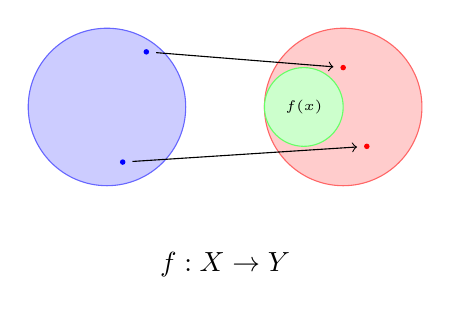
\begin{tikzpicture}
    % draw the sets
    \filldraw[fill=blue!20, draw=blue!60] (-1.5,0) circle (1cm);
    \filldraw[fill=red!20, draw=red!60] (1.5,0) circle (1cm);
    \filldraw[fill=green!20, draw=green!60] (1,0) circle (0.5cm);

    % the texts
    \node at (1,0) {\tiny$f(x)$};
    \node at (0,-2) {$f: X \to Y$};

    % the points in the sets (here I just create nodes to use them later on to position
    % the circles and the arrows
    \node (x1) at (-1,0.7) {};
    \node (x2) at (-1.3,-0.7) {};
    \node (y1) at (1.5,0.5) {};
    \node (y2) at (1.8,-0.5) {};

    % position the elements in the sets (at the nodes we just created)
    \fill[blue] (x1) circle (1pt);
    \fill[blue] (x2) circle (1pt);
    \fill[red] (y1) circle (1pt);
    \fill[red] (y2) circle (1pt);

    % draw the arrows
    \draw[->] (x1) -- (y1);
    \draw[->] (x2) -- (y2);
\end{tikzpicture}
\end{document}

result of above code